\documentclass[a4paper]{report}
\usepackage[utf8]{inputenc}
\usepackage[T1]{fontenc}
\usepackage{RJournal}
\usepackage{amsmath,amssymb,array}
\usepackage{booktabs}

\usepackage{amsmath}
\usepackage{booktabs}
\usepackage{rotating}
\usepackage{multirow}
\usepackage{graphicx}
\usepackage{color}
\usepackage{subcaption}
\usepackage{cite}

\DeclareMathOperator*{\argmaxA}{arg\max} % Jan Hlavacek
\DeclareMathOperator*{\argmaxB}{argmax}   % Jan Hlavacek
\DeclareMathOperator*{\argmaxC}{\arg\max}
\newcommand{\cs}[1]{\texttt{\symbol{`\\}#1}}
\captionsetup{compatibility=false}


\def\bSig\mathbf{\Sigma}
\newcommand{\VS}{V\&S}
\newcommand{\tr}{\mbox{tr}}

%\numberwithin{equation}{section}
%\theoremstyle{plain}
%\newtheorem{thm}{Theorem}[section]
%\newtheorem{proposition}{Proposition}[section]
%\newtheorem{lem}{Lemma}[section]

%% load any required packages here

\begin{document}

%% do not edit, for illustration only
\sectionhead{Contributed research article}
\volume{XX}
\volnumber{YY}
\year{20ZZ}
\month{AAAA}

%% replace RJtemplate with your article
\begin{article}
  % !TeX root = RJwrapper.tex
\title{CopulaTest: An R Package for Copula-Based Bivariate Interval-Censored Data Modeling and Large-Scale Testing}
\author{by Tao Sun, Kevin Anderson and Ying Ding}

\maketitle

\abstract{
In this paper, we introduce an R package named CopulaTest, which implements a novel and computationally efficient estimation method and score test for covariate effect in large-scale bivariate interval-censored data (such as GWAS). We propose a copula-based transformation model with two marginal distributions being approximated by sieves. In doing so, we include both proportional hazards and proportional odds models as special cases. In addition, we use a two-parameter Archimedean copula that is more flexible than Clayton and Gumbel copulas in modeling dependency of two margins. A novel two-step estimation procedure is employed to quickly achieve the final maximum likelihood estimates. Numerical derives are used to approximate the score and observed Fisher information in calculating the score statistics, which is proved to be working well by extensive simulations.
}

\section{Introduction}

Our motivating data come from the Age-Related Eye Disease Study (AREDS), which is a randomized clinical trial of AMD sponsored by the National Eye Institute. Due to intermittent assessment times in this study, the exact time when each eye progressed to late AMD was only known to lie in a certain interval. As a result, the outcome data are bivariate interval-censored. Besides the AREDS data, bivariate interval-censored data commonly exist in many research areas in which two survival times (time to event) are correlated and could not be exactly observed, such as occurrence of kidney diseases.

Copula is a popular approach to model two correlated event times in survival analysis. It models joint survival function by directly building on marginal distributions. Thus, the covariate effect could be conveniently interpreted on a marginal/population level, which is desired in genetic association studies. For bivariate interval-censored data, the existing copula methods only assume a specific dependency structure (i.e. correlation at only the lower tail) or a specific marginal model such as proportional hazards (PH). In addition, there is still no published R package that provides estimation and inference in covariate effect for bivariate interval-censored data under the copula setting.

Let $(T_{1},T_{2})$ be the true bivariate times, with marginal survival functions $S_{1}(t_1)=P(T_1 > t_1)$ and $S_{2}(t_2)=P(T_2 > t_2)$, and joint survival function
$$S(t_{1},t_{2})=P(T_{1} > t_{1}, T_{2} > t_{2}).$$

Assume there are $n$ independent subjects in a study. For subject $i$, we observe $D_i=\{(L_{ij},R_{ij},Z_{ij}), j = 1,2\}$, where $(L_{ij}, R_{ij}]$ is the time interval that $T_{ij}$ lies in. Here, $Z_{ij}$ is a vector of covariates that may affect $T_{ij}$. When $R_{ij} = \infty$, $T_{ij}$ is under right-censoring, and when $L_{ij} = 0$, $T_{ij}$ is under left-censoring.

By the Sklar's theorem (\citeauthor{sklar}, \citeyear{sklar}), as long as the marginal survival functions $S_1$ and $S_2$ are continuous, there exists a unique function $C_\eta$ that connects two marginal survival functions into the joint survival function:
$$S(t_1,t_2) = C_\eta(S_1(t_1),S_2(t_2)),\ t_1, t_2 \geq 0.$$

Here, the function $C_\eta$ is called a copula, which maps the unit square onto [0,1] and its parameter $\eta$ measures the dependency between the two margins. When either $S_1$ or $S_2$ or both become $0$, the copula function becomes $0$ as well. A signature feature of copulas is that they allow dependence structure to be modeled separately from the marginal distributions.

One popular copula family is the Archimedean copula family, which usually has an explicit formula. Two most frequently used Archimedean copulas for correlated survival functions are the Clayton (\citeauthor{clayton}, \citeyear{clayton}) and Gumbel (\citeauthor{gumbel}, \citeyear{gumbel}) copula models, which account for the lower or upper tail dependence between two margins using one univariate parameter.

Here, we consider a more flexible two-parameter Archimedean copula model (\citeauthor{two_param}, \citeyear{two_param}), expressed as:
\begin{equation}
C_{\alpha,\kappa}(u,v)=[1+((u^{-1/\kappa}-1)^{1/\alpha} + (v^{-1/\kappa}-1)^{1/\alpha})^{\alpha}]^{-\kappa}, \ \alpha \in (0,1], \ \kappa \in (0,\infty), \label{two-para-c}
\end{equation}
where $u$ and $v$ are two uniformly distributed margins. The two dependence parameters, $\alpha$ and $\kappa$, are explicitly connected with Kendall's $\tau$, with $\tau = 1- \frac{2\alpha\kappa}{2\kappa + 1}$.

Note that $\alpha$ and $\kappa$ account for the correlation between $u$ and $v$ at both upper and lower tails, respectively. In particular, when $\alpha = 1$, the two-parameter copula (\ref{two-para-c}) becomes the Clayton copula. When $\kappa \rightarrow \infty$, (\ref{two-para-c}) becomes Gumbel copula. Thus, the two-parameter copula model provides more flexibility in characterizing the dependence structure than both Clayton and Gumbel copulas.

With the two-parameter copula, we can write down the joint likelihood function of n subjects:
\begin{align}
\label{joint_likelihood}
L_{n}(S_1, S_2, \alpha,\kappa|D) & = \prod_{i=1}^n Pr(L_{i1} < T_{i1} \leq R_{i1}, L_{i2} < T_{i2} \leq R_{i2}) \nonumber \\ & = \prod_{i=1}^n \biggl[Pr(T_{i1} > L_{i1}, T_{i2} > L_{i2}) - Pr(T_{i1} > L_{i1}, T_{i2} > R_{i2}) \nonumber \\ & \qquad - Pr(T_{i1} > R_{i1}, T_{i2} > L_{i2}) + Pr(T_{i1} > R_{i1}, T_{i2} > R_{i2}) \biggl]  \nonumber \\ & = \prod_{i=1}^n\biggl[C_{\alpha,\kappa}(S_1(L_{i1}),S_2(L_{i2})) - C_{\alpha,\kappa}(S_1(L_{i1}),S_2(R_{i2})) \nonumber \\ & \qquad - C_{\alpha,\kappa}(S_1(R_{i1}),S_2(L_{i2})) + C_{\alpha,\kappa}(S_1(R_{i1}),S_2(R_{i2})) \biggr].
\end{align}
For a given subject $i$, if $R_{ij} = \infty$ (i.e., $T_{ij}$ is right-censored), then any term involving this $R_{ij}$ in the joint survival probability becomes 0. As a result, the joint survival function for subject $i$ will reduce to only 2 or 1 terms.

We use a semiparametric linear transformation model for marginal survival functions:
\begin{equation}
S_{j}(t|Z_j) = \exp(-G_j\{\exp(Z_j^{T}\beta_j)\Lambda_{j}(t)\}), \ j = 1,2, \label{tran_mod}
\end{equation}
where $G_j(\cdot)$ is a pre-specified strictly increasing function, $\beta_j$ is a vector of unknown coefficients, and $\Lambda_{j}(\cdot)$ is an unknown non-decreasing function of $t$. Note that in model (\ref{tran_mod}), the transformation function $G_j(\cdot)$, the regression parameter $\beta_j$ and the infinite-dimensional parameter $\Lambda_j(\cdot)$ are all denoted as margin-specific (indexed by $j$) for generality. In practice, some or all of them can be the same for the two margins and in that case, the corresponding index $j$ can be dropped.

This model (\ref{tran_mod}) contains a class of survival models. For example, when $G_j(x) = x$, the marginal survival function follows a PH model. When $G_j(x) = log(1+x)$, it becomes a PO model. In practice, the transformation can be assumed unknown and get ``estimated'' by the data. For example, two common classes of $G(\cdot)$ function are the Box-Cox transformation $G(x) = [(1+x)^r -1]/r$, $r > 0$, and the logarithmic transformation $G(x) = log(1+rx)/r,$ with $r > 0$. The parameter $r$ can be estimated together with other parameters in the likelihood. The PH or PO model is a special case in both transformation classes.



\section{Sieve Likelihood Approach}
In our likelihood function, we are interested in estimating the unknown parameter $\theta \in \Theta$:
$$\Theta = \{ \theta = (\beta_1, \beta_2, \alpha, \kappa, \Lambda_{1}, \Lambda_{2}) \in \mathcal{B} \otimes \mathcal{M}^1 \otimes \mathcal{M}^2 \}.$$
Here $\mathcal{B}=\{(\beta=(\beta_1,\beta_2), \alpha,\kappa) \in R^p \times R^{(0,1]} \times R^{+},\Vert\beta\Vert + \Vert\alpha\Vert + \Vert\kappa\Vert \leq M\}$ with $p$ being the dimension of $\beta=(\beta_1, \beta_2)$ and $M$ being a positive constant. We denote by $\mathcal{M}^j$ the collection of all bounded and continuous nondecreasing, nonnegative functions over the interval $[c_j,u_j]$, where $0 \leq c_j < u_j < \infty$, $j = 1,2$. In practice, $[c_j,u_j]$ is usually chosen as the range of all $\{L_{ij}\}_{i=1}^n$ and $\{R_{ij}\}_{i=1}^n$.

In our log-likelihood function $l_{n}(\theta|D)=log{L_n(\theta|D)}=\sum_{i=1}^{n}log{L(\theta|D_i)}$, there are finite-dimensional parameters of interest $(\beta,\alpha,\kappa)$ and infinite-dimensional nuisance parameters $(\Lambda_{1},\Lambda_{2})$, which need to be estimated simultaneously. Unlike the right-censored data, the interval-censored data do not apply tools like partial likelihood and martingale due to the absence of exact event observations. Instead, following \citet{univariate_PO_sieve}, we employ the sieve approach and form a sieve likelihood. Specifically, similarly as in \citet{frailty_case_II_transformation_sieve}, we use Bernstein polynomials to build a sieve space $\Theta_n = \{ \theta_n = (\beta, \alpha, \kappa, \Lambda_{1n}, \Lambda_{2n}) \in \mathcal{B} \otimes \mathcal{M}_{n}^1 \otimes \mathcal{M}_{n}^2 \}$. Here, $\mathcal{M}_n^j$ is the space defined by Bernstein polymials:
$$\mathcal{M}_n^j = \{ \Lambda_{jn}(t) = \sum_{k=0}^{m} \phi_{jk}B_{k}(t,m,c_j,u_j): \sum_{0 \leq k \leq m} |\phi_{jk}| \leq M_{n}, \ 0 \leq \phi_{j0} \leq \phi_{j1} \leq ... \leq \phi_{jm} \},$$
where $B_{k}(t,m,c_j,u_j)$ represents the Bernstein basis polynomials defined as:
\begin{equation}
B_{k}(t,m,c_j,u_j) =  {m \choose k} (\frac{t-c_j}{u_j-c_j})^{k} (1-\frac{t-c_j}{u_j-c_j})^{m-k}, \ k = 0,...,m, \label{Bern}
\end{equation}
with degree $m = o(n^{v})$ for some $v \in (0,1), \ j=1,2$.

The use of Bernstein polynomials naturally fits the interval-censored data as they are built based on intervals. One advantage of Bernstein polynomials is that they do not require the specification of interior knots, as seen from (\ref{Bern}), making them easier to work with. Another great advantage of Bernstein polynomials is that they can naturally achieve the non-negativity and monotonicity properties of $\Lambda_1(t)$ and $\Lambda_2(t)$ through reparameterization, as discussed in \citet{frailty_case_II_transformation_sieve}. \textbf{add reparameterization strategies}.

With the sieve space defined above, the infinite-dimensional parameters $\Lambda_j(t)$  will be approximated by $\Lambda_{jn}(t) \in \mathcal{M}_n^j$. In the next section, we propose an estimation procedure to maximize $l_n(\theta|D)$ over the sieve space $\Theta_n$ to obtain the sieve MLE $\hat{\theta}_n = (\hat{\beta}_n, \hat{\alpha}_n, \hat{\kappa}_n, \hat{\Lambda}_{1n}, \hat{\Lambda}_{2n})$.


\section{Estimation and Test Procedure}
\citet{two_stage_right_censor} and \citet{two_stage_interval_censor} proposed two-step estimation procedures for the dependence parameter in a copula function for bivariate right-censored and interval-censored data, respectively. In essence, each $S_1$ and $S_2$ is estimated marginally in step 1. Then their estimators are plugged into the joint likelihood (i.e., the copula function) to form a pseudo-likelihood. In step 2, the dependence parameter is estimated through maximizing the pseudo-likelihood function with respect to the dependence parameter only. Both \citet{two_stage_right_censor} and \citet{two_stage_interval_censor} were only interested in the inference of the dependence parameter, and they have shown that the estimator from step 2 is consistent and asymptotically normal. In our case, we are also interested in the inference of the regression parameter $\beta$. We extend their ideas to obtain the full sieve MLE $\hat{\theta}_n$ as follows:
\begin{enumerate}
\item Obtain initial estimates of $\theta_n$:
\begin{enumerate}
\item $(\hat{\beta}_{jn}^{(1)}, \hat{\Lambda}_{jn}^{(1)}) = \argmaxC\limits_{(\beta_j, \Lambda_{jn})} l_{jn}(\beta_j, \Lambda_{jn})$, where $l_{jn}$ denotes the sieve log-likelihood function for the marginal model, $j=1, 2$;
\vspace{0.1cm}
\item $(\hat{\alpha}_{n}^{(1)},\hat{\kappa}_{n}^{(1)})=\argmaxC\limits_{(\alpha,\kappa)} l_n(\hat{\beta}_{n}^{(1)}=(\hat{\beta}_{1n}^{(1)},\hat{\beta}_{2n}^{(1)}), \alpha, \kappa, \hat{\Lambda}_{1n}^{(1)},\hat{\Lambda}_{2n}^{(1)})$, where $\hat{\beta}_{jn}^{(1)}$ and $\hat{\Lambda}_{jn}^{(1)}$ are the initial estimates obtained from (a), and $l_n$ is the joint sieve log-likelihood.
\end{enumerate}
%The dependency parameter estimates obtained by step 1 are already asymptotically consistent and normal, though their variance-covariance estimates could be solved directly from the hessian matrix (Sun 2006).
\vspace{0.2cm}
\item Simultaneously maximize the joint sieve log-likelihood to get final estimates:\\
$\hat{\theta}_n = (\hat{\beta}_n,\hat{\alpha}_n,\hat{\kappa}_n,\hat{\Lambda}_{1n},\hat{\Lambda}_{2n})=\argmaxC\limits_{(\beta,\alpha,\kappa,\Lambda_{1n},\Lambda_{2n})} l_n(\beta,\alpha,\kappa,\Lambda_{1n},\Lambda_{2n})$ with initial values \\ $(\hat{\beta}_{n}^{(1)},\hat{\alpha}_{n}^{(1)},\hat{\kappa}_{n}^{(1)},\hat{\Lambda}_{1n}^{(1)},\hat{\Lambda}_{2n}^{(1)})$, obtained from step 1.
\end{enumerate}

Note that the initial estimates from step 1 are already consistent. Step 2 produces correct variance covariance estimates for all the parameters using the joint sieve likelihood. Our experience finds that, the performance of convergence is greatly improved by starting with the initial values from step 1 in the (simultaneous maximization) step 2. 

For the inference of specific covariate effect (i.e. SNP effect in the GWAS setting), we will focus on the score test due to computational efficiency, as one only need to estimate the parameter once (under the null hypothesis that the SNP is not associated with the outcome), which is much less computationally intensive as compared to the likelihood ratio test or Wald test (Table \ref{tab:test_compare}).

\section{Implementation in R}
The R package \textbf{CopulaTest} implements the proposed estimation and test method above and is now located at CRAN. Following the command below in R console will start the installation of the package:

\begin{example}
  > install.packages("CopulaTest")
\end{example}

The Newton-Raphson algorithm can be applied to obtain the initial values in step 1(a) and the conjugate gradient algorithm can be employed on the joint sieve log-likelihood in steps 1(b) and 2. \textbf{discuss how NR algorithm fails in steps 1b and 2}.

There are four main functions in the \textbf{CopulaTest} package: a parametric estimation function \texttt{ic\_par\_copula} that gives estimates, se, Wald statistics, p value and other objects to be applied to the score test procedure, a parametric score test function \texttt{ic\_par\_copula\_score} that takes in the null hypothesis object from \texttt{ic\_par\_copula} and perform score test for targeted covariates, a semiparametric estimation function \texttt{ic\_sp\_copula} that implements the semiparametric models for margins and outputs similar results as \texttt{ic\_par\_copula}, and the last function \texttt{ic\_sp\_copula\_score} that operates similarly as \texttt{ic\_par\_copula\_score}.

First, we will briefly introduce the options in \texttt{ic\_sp\_copula}:

\begin{example}
  ic_sp_copula(copula = "Copula2", m = 3, r = 1, data, var_list, l = 0, u, iter = 200, 
               stepsize = 1e-05, method = "NR")
\end{example}

The \texttt{copula} argument defines the type of copula model to be fitted, including Clayton, Gumbel and Copula2 (two-parameter copula). The integer \texttt{m} is the Bernstein polynomial degree, with default $m=3$. \texttt{r} corresponds to the linear transformation function, with $\texttt{r} = 1$ (default) for PH and $\texttt{r} = 3$ for PO. The arguments \texttt{data} and \texttt{var\_list} contain the date frame and a vector of covariate names to be fitted. The parameters $\texttt{l}$ and $\texttt{u}$ form the range of all endpoints of observed intervals. By default, we set $\texttt{l} = 0$. Based on our experience, we usually choose $\texttt{u}$ as the largest non-infinity endpoint plug a small constant. The default optimization method for estimation and score test is Newton Raphson, with \texttt{method} = ``NR''.  The options for optimization are \texttt{iter} for the maximum iteration steps and \texttt{stepsize} for iteration stepsize, with default settings at $200$ and $1e-05$, respectively. Note that we realize the Conjugate Gradient (CG) algorithm may give more accurate SE than NR when \texttt{copula} = ``Copula2". So we provide an alternative option \texttt{method} = ``CG'' when ``Copula2" is applied. The computing speed of ``CG" is much lower than that in ``NR". The output is an object, which is a list of detailed objects such as a summary of covariate effects with wald statistics and p values, as well as other objects to be applied for the score test in \texttt{ic\_sp\_copula\_score}.

If we fit a null model using \texttt{ic\_sp\_copula}, then we can directly use its output object to perform score test using \texttt{ic\_sp\_copula\_score}:

\begin{example}
  ic_sp_copula_score(object, var_score)
\end{example}

The \texttt{object} argument take direct output from the null model fitted by the function \texttt{ic\_sp\_copula}. The \texttt{var\_score} argument is a vector of covariate(s) to be tested by the score test.

Tables \ref{tab:effect_m}, \ref{tab:effect_covariate_num}, \ref{tab:effect_sample_size} and \ref{tab:effect_right_censor} evaluate the computing speed of the two-parameter copula sieve model in performing 1000 score tests under a simulated GWAS setting. Table \ref{tab:test_compare} compares speed of Wald, LRT and score tests. The optimization method is Newton-Raphson.

In addition, we provide predicted joint survival probability based on a fitted copula-sieve model (\texttt{surv2\_sieve}) and plot a corresponding three-dimensional joint survival function by \texttt{plot3d\_sieve}. 

\begin{table}[htbp]
\centering
\caption{Effect of Bernstein polynomial degree on computing speed. Sample size = 500. Number of covariates in null model = 3. Right-censoring rate = 25\%.}
\label{tab:effect_m}
\resizebox{0.5\linewidth}{!}{ % Resize table to fit within \linewidth horizontally
\begin{tabular}{clllll}
\toprule
\multicolumn{1}{l}{m}     & $2$   & $4$  & $6$  &  $8$ & $10$          \\
\hline
\multicolumn{1}{l}{time (s)}   & 544   & 760    &   1071        &   1407             & 1863                       \\
\bottomrule
\end{tabular}%
}

\bigskip
\vspace{0.1cm}

\caption{Effect of covariate number on computing speed. Sample size = 500, Bernstein degree $m=4$. Right-censoring rate = 25\%.}
\label{tab:effect_covariate_num}
\resizebox{0.6\linewidth}{!}{ % Resize table to fit within \linewidth horizontally
\begin{tabular}{clllll}
\toprule
\multicolumn{1}{l}{Covariate number}     & $4$   & $6$  & $8$  &  $10$ & $12$          \\
\hline
\multicolumn{1}{l}{time (s)}   & 935   & 1231    &   1615        &   2022             & 2251                       \\
\bottomrule
\end{tabular}%
}

\bigskip
\vspace{0.1cm}

\caption{Effect of sample size on computing speed. Number of covariates = 4, Bernstein degree $m=4$. Right-censoring rate = 25\%.}
\label{tab:effect_sample_size}
\resizebox{0.6\linewidth}{!}{ % Resize table to fit within \linewidth horizontally
\begin{tabular}{cllllll}
\toprule
\multicolumn{1}{l}{Sample size}     & $200$   & $400$  & $800$  &  $1000$ & $2000$    & $5000$      \\
\hline
\multicolumn{1}{l}{time (s)}   & 477   & 718    &   1386        &   1254             & 3031      &        6977         \\
\bottomrule
\end{tabular}%
}

\bigskip
\vspace{0.1cm}

\caption{Effect of right-censoring rate on computing speed. Sample size = 4. Number of covariates = 4. Bernstein degree $m=4$.}
\label{tab:effect_right_censor}
\resizebox{0.6\linewidth}{!}{ % Resize table to fit within \linewidth horizontally
\begin{tabular}{cllll}
\toprule
\multicolumn{1}{l}{Right-censoring rate}     & $10\%$   & $25\%$  & $50\%$  &  $75\%$       \\
\hline
\multicolumn{1}{l}{time (s)}   & 593   & 603    &   608        &   602    \\
\bottomrule
\end{tabular}%
}

\bigskip
\vspace{0.1cm}

\caption{Comparison of Wald, score and Likelihood-ratio tests on computing speed under the same Null hypothesis. Sample size = 4. Number of covariates = 4. Bernstein degree $m=4$. Right-censoring rate = 25\%.}
\label{tab:test_compare}
\resizebox{0.4\linewidth}{!}{ % Resize table to fit within \linewidth horizontally
\begin{tabular}{clll}
\toprule
\multicolumn{1}{l}{Types}     & Wald   & LRT  & Score       \\
\hline
\multicolumn{1}{l}{time (s)}   & 2219   & 2215    &   604       \\
\bottomrule
\end{tabular}%
}
\end{table}

\section{Examples}
\begin{example}
 #load data
 df <- data(clayton_weibull_PH) #example data frame included in /copulaTest/data
 
 #fit a Clayton-Weibull model under PH
 fit_clayton_weibull_ph <- ic_par_copula(data=df,copula="Clayton",m.dist="Weibull",
 m.model="PH",var_list=c("x1","x2","x3"))
 
 #running parametric score test
 fit_clayton_weibull_ph2 <- ic_par_copula(data=df,copula="Clayton",m.dist="Weibull"
 ,m.model="PH",var_list=c("x1","x2"))
 score_clayton_weibull_ph <- ic_par_copula_score(object=fit_clayton_weibull_ph2,var
 _score=c("x3"))
 
 #fit a sieve-based semiparametric Copula2 model under PH
 fit_copula2_sieve_ph <- ic_sp_copula(data=df,copula="Copula2",m=3,r=1,l=0, u=17,var
 _list=c("x1","x2","x3"), iter=300, method = "CG")
 
 #semi parametric score test
 fit_copula2_sieve_ph2 <- ic_sp_copula(data=clayton_weibull_PH,copula="Copula2",m=3,
 r=1,l=0, u=17, var_list=c("x1","x2"), iter=200, method="CG")
 score_copula2_sieve_ph <- ic_sp_copula_score(object=fit_copula2_sieve_ph2, 
 var_score=c("x3"))
\end{example}

 Figure~\ref{figure:3D} is a predicted joint survival probability plot, based on a fitted copula sieve model.
\begin{figure}[htbp]
  \centering
  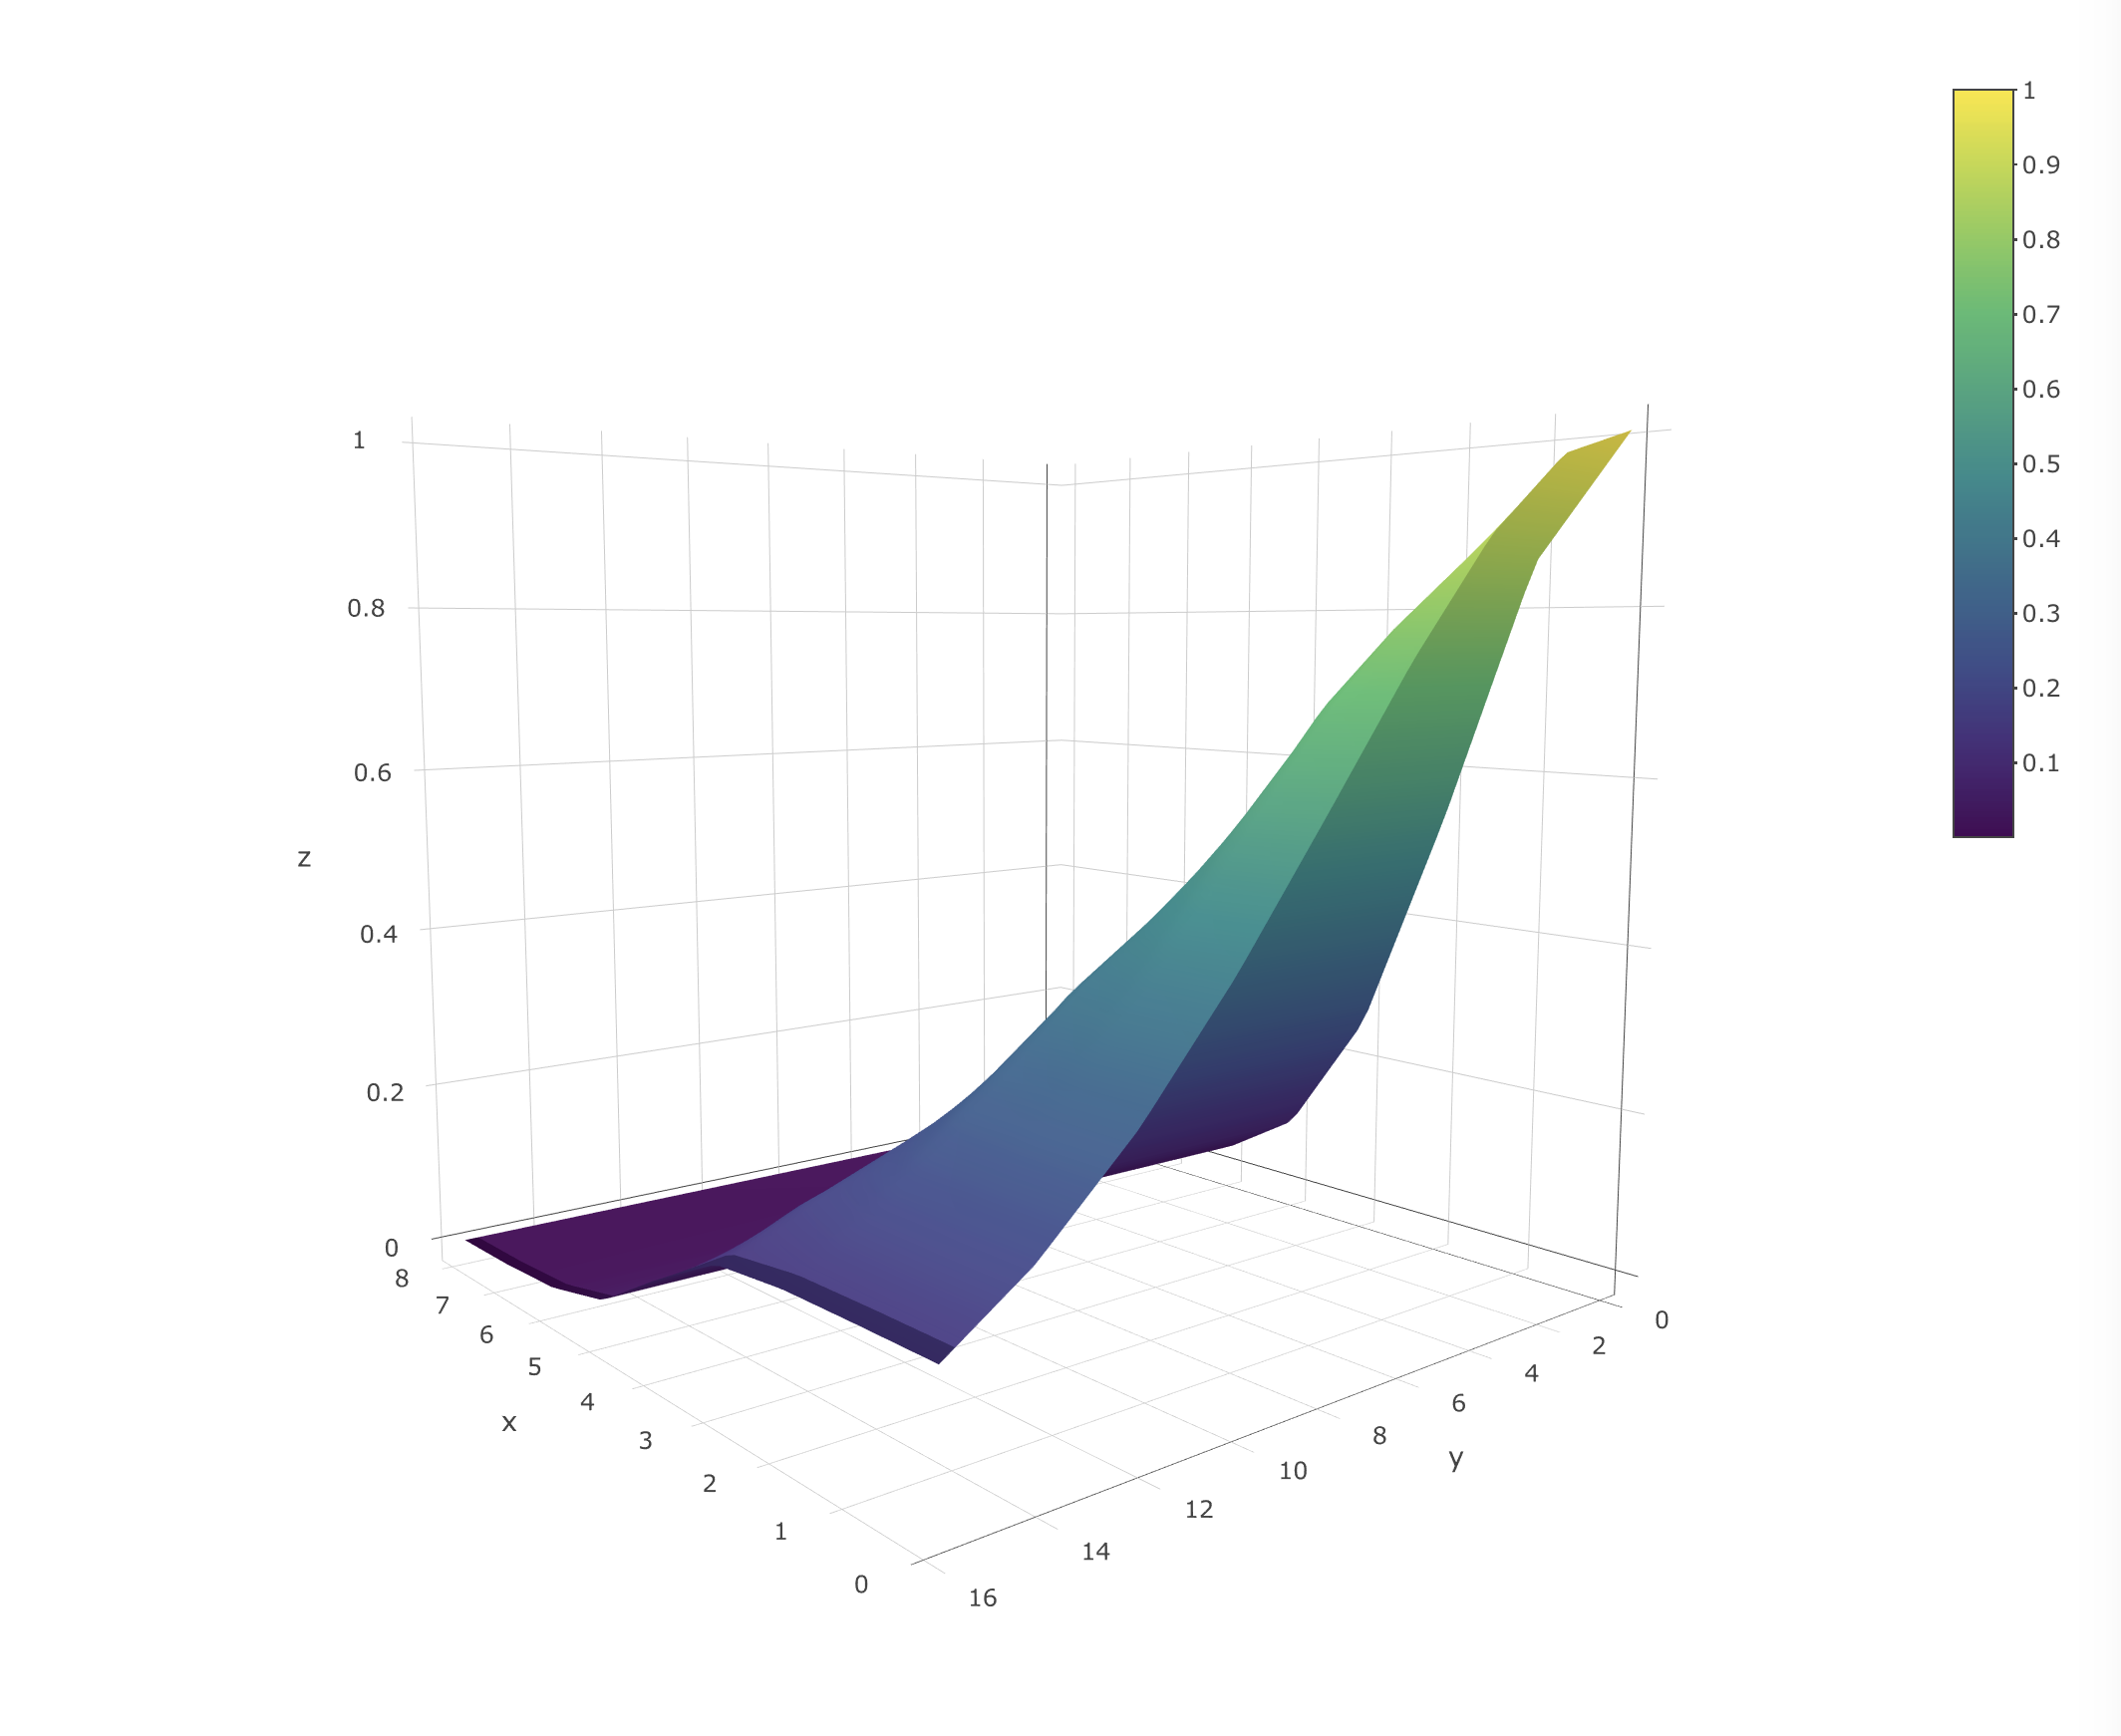
\includegraphics[scale=0.3]{3D.png}
   \caption{Predicted joint survival probability}
  \label{figure:3D}
\end{figure}

\section{Summary}
The motivation of the our work is to identify significant genetic variants associated with the progression to late-AMD, using high-dimensional bivariate interval-censored data. Most existing studies only focused on a small set of known AMD risk variants and treated the (right) interval endpoint as the true event time. Here we present a two-parameter copula model for bivariate interval-censored data, with margins under semiparametric transformation models that include PH and PO. The two-parameter copula model has two dependency parameters, accounting for marginal dependency at both tails, and regards Clayton and Gumbel copulas as special cases. For estimation, we use Bernstein polynomials to build a sieve log-likelihood and propose a two-step procedure to quickly achieve the MLEs. Further, we demonstrate asymptotic consistency, normality and efficiency for these sieve MLEs. For the inference of covariate effect, particularly in the high-dimensional setting, we employ a computationally efficient score test, which approximates the score function and Fisher information matrix by numerical derivatives. Simulation results indicate this numerical approach works well. All estimation and test procedures have been built in an R package ``CopulaTest'', which is located on the CRAN.

\bibliography{CopulaTest}

\address{Tao Sun\\
  University of Pittsburgh\\
  130 De Soto Street\\
  United States\\
  (ORCiD if desired)\\
  \email{tao.sun@pitt.edu}}

\address{Kevin Andersen\\
  University of Pittsburgh\\
  130 De Soto Street\\
  United States\\
  (ORCiD if desired)\\
  \email{kja34@pitt.edu}}

\address{Ying Ding\\
  University of Pittsburgh\\
  130 De Soto Street\\
  United States\\
  (ORCiD if desired)\\
  \email{yingding@pitt.edu}}

\end{article}

\end{document}
